% Chapter Template

\chapter{Theory} % Main chapter title

\label{Chapter3} 

%----------------------------------------------------------------------------------------
%	SECTION 1
%----------------------------------------------------------------------------------------

\section{Static site generators}

Static site generators take your app and build it before serving to users. 
This means users receive plain HTML files. This moves a large computational burden from run time to build time which results in significantly faster load times for users.
Furthermore, this approach allows for more aggressive and efficient caching.

\subsection{Nextjs}

Nextjs\footnote{https://nextjs.org/} is a React framework. Not explicitly a static site generator but has support for it. 
Nextjs has support for a ton of interesting features, 

\begin{itemize}
	\item Image optimization
	\item Hybrid static site generation and server side rendering
	\item Internationalization
	\item Typescript support
\end{itemize}

It is important to note that Nextjs heavily uses server side rendering. If used in the end result, the deployment should support this. 
This can be achieved by using Lambda, Lambda@edge or Cloudfront functions.  

\subsubsection{Serverless server side rendering}

As noted, Nextjs uses server side rendering. 
This improves performance as it allows the server to render a page instead of the client.
Servers can have a lot more computing power than the average consumer workstation or mobile.

This does mean that a lot of round-trips will happen between the client and the server. 
Since performance is a key component of the solution here, the solution should try to minimize this.

Luckily, AWS offers a few solutions for this. 
The simplest solution is to use regular lambda functions. 
This will work fine, however the location where this lambda function runs might be very far away from the client, resulting in a larger than desired network latency.
This can be mitigated by using the Lambda@Edge technology from AWS. Instead of running the lambda function in the main AWS data center, it instead runs in the regional edge location.
Regional edge locations are significantly closer to the user, which helps with latency but it is still far removed.
Going one step further, AWS also offers Cloudfront functions. These are functions that run the closest to the client as currently possible.

\begin{figure}[htb!]
	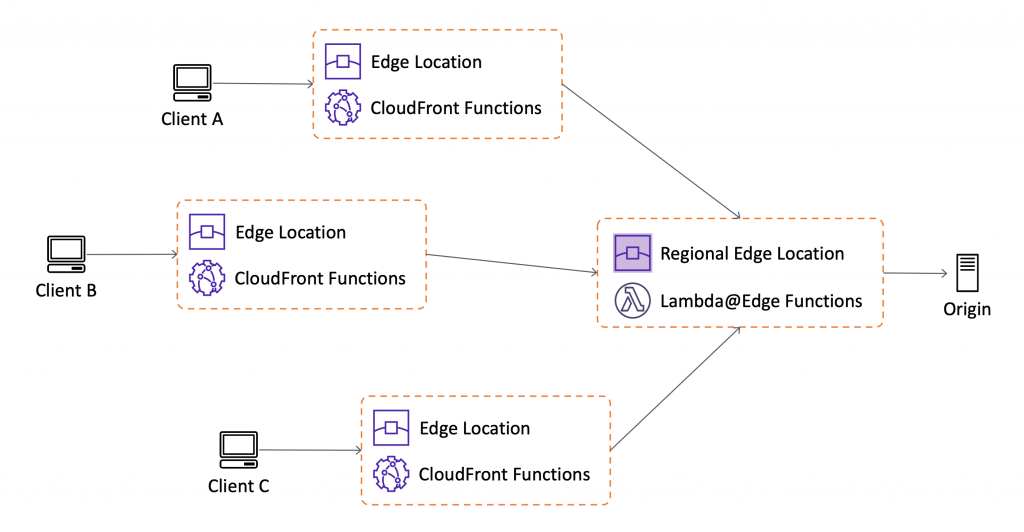
\includegraphics[scale=0.5]{@edge}{}
	\caption{AWS solutions for running code @edge \cite*{aws@edge}}
	\label{fig:@edge}
\end{figure}


\subsection{Gatsby}

Gatsby\footnote{https://www.gatsbyjs.com/} is a static site generator at heart. It is one of the most popular frameworks around \cite{jamstackorg-generators}

\begin{itemize}
	\item Static site generation leads to better performance
	\item Image optimization
	\item Large plugin ecosystem
\end{itemize}



\section{Cypress}

Cypress\footnote{https://www.cypress.io/} is a tool made to run automated end-to-end tests in a browser. 

This research will use Cypress for it's simple API to control browsers programmatically. It will allow us to define the performance benchmarks as code and easily run that on the different PoC applications.

\section{Strapi}

Strapi\footnote{https://strapi.io/} is an open-source CMS. While Stampix uses a different CMS, this research chose Strapi because it is easy to run locally. 
Because the pipeline is running the CMS locally, it is much easier to create a configuration that the pipeline can reuse across different deployments. 


\section{Docker}

Docker\footnote{https://www.docker.com/} is a tool to run and manage containers. All of the components of our benchmarking pipeline will be "Dockerized": the PoC applications, Strapi and even Cypress. 
By using containers for this, pipelines can be created that are platform independent. 
You, the reader, can run the benchmark on your own computer and you will see similar results as presented in this paper. This is explained more thoroughly in chapter \ref{Chapter4}


\section{Methodology}

To make an educated decision on what framework provides the best performance, a benchmarking pipeline will be created. 
Small, proof of concept applications will be created in the above mentioned frameworks which try to replicate real world behavior as close as possible.

Each PoC application must at least be able to load some assets from the CMS and perform an API request to the backend.


\section{Metrics}

Now that it is defined how this performance benchmark will be created and ran, key metrics can be defined.

\subsection{Largest contentful paint}

\begin{quote}
	Largest Contentful Paint (LCP) is an important, user-centric metric for measuring perceived load speed because it marks the point in the page load timeline when the page's main content has likely loaded—a fast LCP helps reassure the user that the page is useful.
	\hfill \cite{webvitalswebsite}
\end{quote}

LCP is an important metric for us. In the original application, this would happen after the request to the CMS. 
That means LCP will be rather late for the average use.
By using static site generators, it can be assured that all of the content shown to users is served from a very fast CDN. 

\subsection{First input delay}

\begin{quote}
	First Input Delay (FID) is an important, user-centric metric for measuring load responsiveness because it quantifies the experience users feel when trying to interact with unresponsive pages—a low FID helps ensure that the page is usable.
	\hfill \cite{webvitalswebsite}
\end{quote}

FID is a very important metric. When a user visits the website, they want to see content and interact with the site as quick as possible. 
When a site has a large FID, it means users have to waste precious time waiting for the site to fully load. In the performance benchmark, this is measured by total blocking time. 

\subsection{Bundle size}

When a user visits the site, one of the main reasons they have to wait for a site to load is network connectivity. 
If a user has a faster network connection, they can download the static files of the website faster.
This is a part of the system where Stampix has very little control, it is impossible to give the users a better network connection. 
However, what can be done, is make sure that the user has to download the smallest amount of data as possible. 
To achieve this, a technique called minification can be used to take our front end code and make it smaller.

Code written by developers might look something like:

\begin{verbatim}
    function doSomething(parameterName) {
        const aVariableWithALongName = 'foo'
        return aVariableWithALongName + parameterName + 'bar'
    }
\end{verbatim}

After minification, the code will look something like:

\begin{verbatim}
    function a(o){return"foo"+o+"bar"}
\end{verbatim}

Over the entire codebase, shortening the code like this will result in a significantly smaller download size for the user.
